\documentclass[12pt]{article}
\usepackage{graphicx} % This lets you include figures
%\usepackage{hyperref} % This lets you make links to web locations
\graphicspath{ {./images/} }
\usepackage[normalem]{ulem}  % для зачекивания текста
\usepackage{color} % подключить пакет color
% выбрать цвета
\definecolor{BlueGreen}{RGB}{49,152,255}
\definecolor{Violet}{RGB}{120,80,120}
% назначить цвета при подключении hyperref
\usepackage[unicode, colorlinks, urlcolor=BlueGreen, linkcolor=Violet, pagecolor=Violet]{hyperref}
%отступы
\usepackage[left=3cm,right=3cm,top=2cm,bottom=3cm,bindingoffset=0cm]{geometry}
\setlength{\parindent}{5ex}

%Русский язык
\usepackage[T2A]{fontenc} %кодировка
\usepackage[utf8]{inputenc} %кодировка исходного кода
\usepackage[english,russian]{babel} %локализация и переносы

\usepackage[rightcaption]{sidecap}
\usepackage{subcaption}
\usepackage{wrapfig}

\usepackage{float}

\usepackage{imakeidx}

\makeindex

\title{Автоматическая система полива домашних растений. Руководство по эксплуатации}
\author{Сериков Василий}

\begin{document}
	\begin{titlepage}
		\begin{center}
			\textsc{Федеральное государственное автономное образовательное учреждение высшего образования«Московский физико-технический институт (национальный исследовательский университет)»\\[5mm]
			}
			\vfill
			\textbf{Автоматическая система полива домашних растений. Руководство по эксплуатации}
			
		\end{center}
	
	\vfill
	\begin{center}
		Москва, 2023 г.
	\end{center}
	\end{titlepage}
	
	\tableofcontents
	
	\clearpage
	\newpage
	
	\section{Об этом устройстве}
	\subsection{Правила безопасности}
	
	Автоматическая система полива домашних растений (далее устройство)\\
	
	\textbf{ВНИМАНИЕ!}\\
	
	$\cdot$ Внимательно прочитайте эту инструкцию перед установкой и эксплуатацией устройства, если у вас возникнут вопросы обращайтесь
	к официальному производителю. \\
	
	$\cdot$ Используйте прибор только по назначению
	указанному в данной инструкции.\\
	
	$\cdot$ Устройство должно быть установлено с соблюдением
	существующих местных норм и правил эксплуатации
	электрических сетей.\\
	
	$\cdot$ Не подключайте и не отключайте устройство
	от электрической сети, вынимая вилку из розетки, используйте переключатель ВКЛ/ВЫКЛ.\\
	
	$\cdot$ Перед установкой устройства убедитесь,
	что параметры электрической сети
	соответствуют параметрам, указанным в разделе Характеристики \\
	
	$\cdot$ Устройство должно находится вдали от резервуара с водой (попадание воды может вызвать короткое замыкание).\\
	
	$\cdot$ Производить настройку режимов согласно инструкции (см. пункт Начало работы).\\
	
	$\cdot$ Производить разборку корпуса для модернизации должен квалифицированный специалист в области радиоэлектроники.\\
	
	$\cdot$ Беречь от детей (!).\\
	
	\subsection{Описание}
	
	Устройство представляет собой систему из набора электронных модулей и радиотехнических элементов, управляемых микроконтроллером. Данное устройство позволяет в режиме реального времени подавать с заданными пользователем частотой и продолжительностью воду с помощью водяных помп из резервуара непосредственно в горшки с цветами. Особенностью данного устройства является наличие двух помп для полива растений с различным потреблением воды.
	
	Также данное устройство можно собрать самостоятельно по пунктам в разделе Инструкция по самостоятельной сборке.
	
	\subsection{Комплектация}
	Данное устройство состоит из следующих компонентов:
	\begin{enumerate}
		\item Пластиковый корпус - 1шт.
		\item Помпа водяная - 2шт.
		\item Экран жидкокристаллический (lcd 1602 I2C) - 1шт.
		\item Энкодер (HC11) - 1шт.
		\item Кнопка тактовая - 1шт.
		\item Переключатель двухпозиционный - 1шт.
		\item Микроконтроллер (Arduino Nano ATmega328P) - 1шт.
		\item Транзистор полевой (IRF1407) - 2шт.
		\item Резистор 10к$\Omega$ - 2шт.
		\item Резистор 200$\Omega$ - 2шт.
		\item Диод 1N5408 - 2шт.
	\end{enumerate}
	
	\subsection{Технические характеристики}
	Данное устройство обладает следующими параметрами: \\
	
	$-$ Напряжение питания - 4.7-5.5 В \\

	$-$ Масса - \\
	
	$-$ Габариты - \\
	
	$-$ Количество поддерживаемых различных растений - 2 (или больше см. пункт Модернизация) \\
	
	$-$ Шаг по времени настройки интервала между включениями помпы - h (час) \\
	
	$-$ Шаг по времени настройки интервала работы помпы - m (минута)\\
	
	$-$ Расход воды помпой -  л/ч \\
	
	
	
	
	\section{Начало работы}
	
	
	\section{Инструкция по самостоятельной сборке}
	
	Данный пункт поможет тем, кто хочет собрать данное устройство самостоятельно.
	\begin{enumerate}
		\item Для начала необходимо приобрести все элементы указанные в главе Комплектация (примечание: пластиковый корпус необходимо напечатать на 3Д принтере, модель корпуса и STL находятся в папке body model на github).
		
		\item Далее надо соединить все компоненты по следующей схеме:
		
		\begin{figure}[H]
			\center{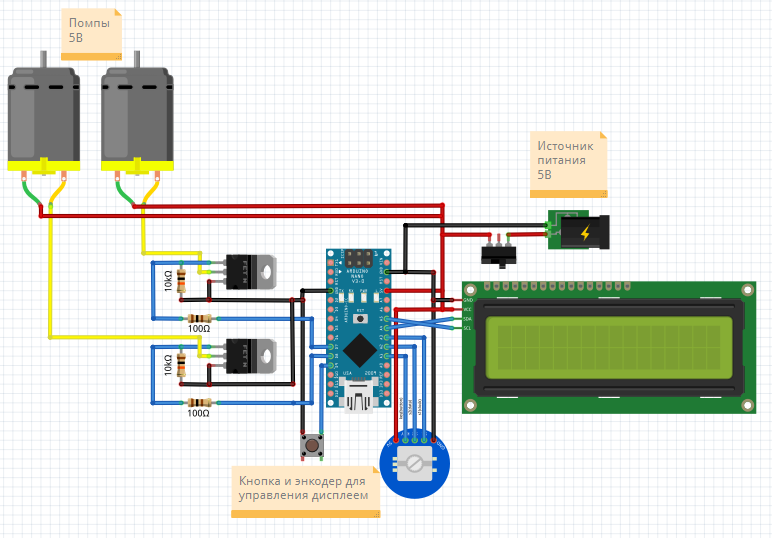
\includegraphics[scale=1]{../pictures/scheme.png}}
			\caption{Схема устройства}
		\end{figure}
		Для этого вам понадобятся паяльные принадлежности, термоусадка и провода.
		
		\item Следующий пункт - установка среды программирования Arduino IDE, компиляция и загрузка прошивки на контроллер. Про установку Arduino IDE, драйверов и про все остальные предварительные ласки рекомендую почитать на сайте \href{https://alexgyver.ru/arduino-first/#Arduino_IDE}{Алекса Гайвера}

	\end{enumerate}
	
\end{document}